The pitch detector will be made for usage on the web. The web is chosen for portability and ease of use. The end user, be it an individual wanting to learn to sing or a choir testing candidates, can use any mobile device with a microphone, be it a laptop, tablet or smartphone, and without installing anything test the accuracy of their singing or tune their guitar.

\subsection{Web Audio API}
As the pitch detector is intended to be used in the browser, for portability and ease of use, the Web Audio API will be extensively used. The purpose of the API is to allow developers control over audio processing functionality on browsers, by providing access to user audio devices, adding effects and more. 
The Web Audio API operates in an AudioContext, which can be thought of as an empty control flow graph. The graph is constructed using AudioNodes which fall into one of three categories: input or source nodes, modifier nodes or output nodes. The nodes are then connected to each other to form the graph. 

The graph operates by passing blocks of data (called render quanta) between nodes, where one render quantum consists of frames of samples, where one frame contains one sample for every audio channel, at least according to the W3C Audio API 1.1 specifications. Render quantum seems to be a term reserved for the low-level processing of the data passing between nodes, and in reality is (at least on tested browsers) not an array of frames with a sample per channel but rather a set of channels with contiguous samples. Regardless of the internal memory layout of the blocks, important to note is that the stream consists of blocks of data, which will be called render quanta for a lack of naming at API level, and are fixed in size. The render quantum size on Firefox is 128 and has not been tested on other browsers. The pitch detector does however seem to work with this assumption, at least on Google Chrome.

%https://www.w3.org/TR/webaudio/#rendering-loop

\subsubsection{Sources and destinations}
The source nodes, as the name implies, are entry points for the audio control graph, they provide signals. Some of these include the OscillatorNode, a node which produces pure sinusoids, and MediaElementAudioSourceNode, which uses the media in an existing HTML audio element. As the purpose of the application is for the user to be able to record their own singing and have it analyzed for pitch correctness, the source in this case will be a MediaStreamAudioSourceNode, which provides a source signal from a MediaStream. The actual source will the method navigator.mediaDevices.getUserMedia\(\) that provides the MediaStream, but this is technically outside the AudioContext so it is not a source node.

The output may be either the user's system's speakers, or another MediaStream. In this case, there will not be an output node because it is simply not needed. The output will be the result of the Fourier analysis.

\subsubsection{Modifiers} 
The modifier nodes are the nodes that are neither sources nor destinations, they take in the signal from a node, performs some transformation on the signal, and then hands it over to the next node, or nodes, in the graph. Some of these nodes apply effects, like reverb or gain. Others may be used to visualize audio or split audio into separate channels for per-channel modification.

The available modifiers unfortunately do not help with the development of the pitch detector, so a lot of the processing would be done with Worklet nodes, a node that allows custom functionality. With this in mind, the simplest way may be to not use the Audio API audio graph, but to just take the output from the microphone and in the simplest possible way turn it into data to be processed using regular procedural programming. The AnalyserNode has Fourier transform capabilities, but there does not seem to be a way to zero-pad it, which is integral to achieving both real-time processing and enough frequency resolution for base singers. 

\subsection{Pitch detector architecture}
The identified steps of the pitch detector at the highest level are input, zero-padding, FFT, peak picking and some post-processing. It is a simple pipeline of collecting enough samples for the FFT from a microphone and then running analysis on the spectrum data. The only problem at this stage is converting the stream from the microphone to something that can be processed. There seems to be mainly two ways to go about implementing this kind of conversion. One way is to feed the stream from the microphone into a recorder and decode the binary data that becomes available with time. The other is to handle the raw audio data on the audio rendering thread by building a custom audio processor that handles the processing, whatever that may be. 

As the Fourier transform and any peak-picking algorithm of choice works in the frequency domain, using the audio graph does not make much sense. The only thing the audio graph would be responsible for would be moving the render quanta between nodes, but this is a bit like using a chainsaw to slice bread. Figure \ref{fig:pdArch} shows the proposed architecture which uses a bridge node to send the raw audio data from the rendering thread to the main thread. For every render quanta processed the data is passed through the node-processor port from the processor to the node in the main thread where it is passed from the node to a callback function. This callback function may then be used to accumulate the render quanta and start analysis.

\begin{figure}[ht]
    \centering
    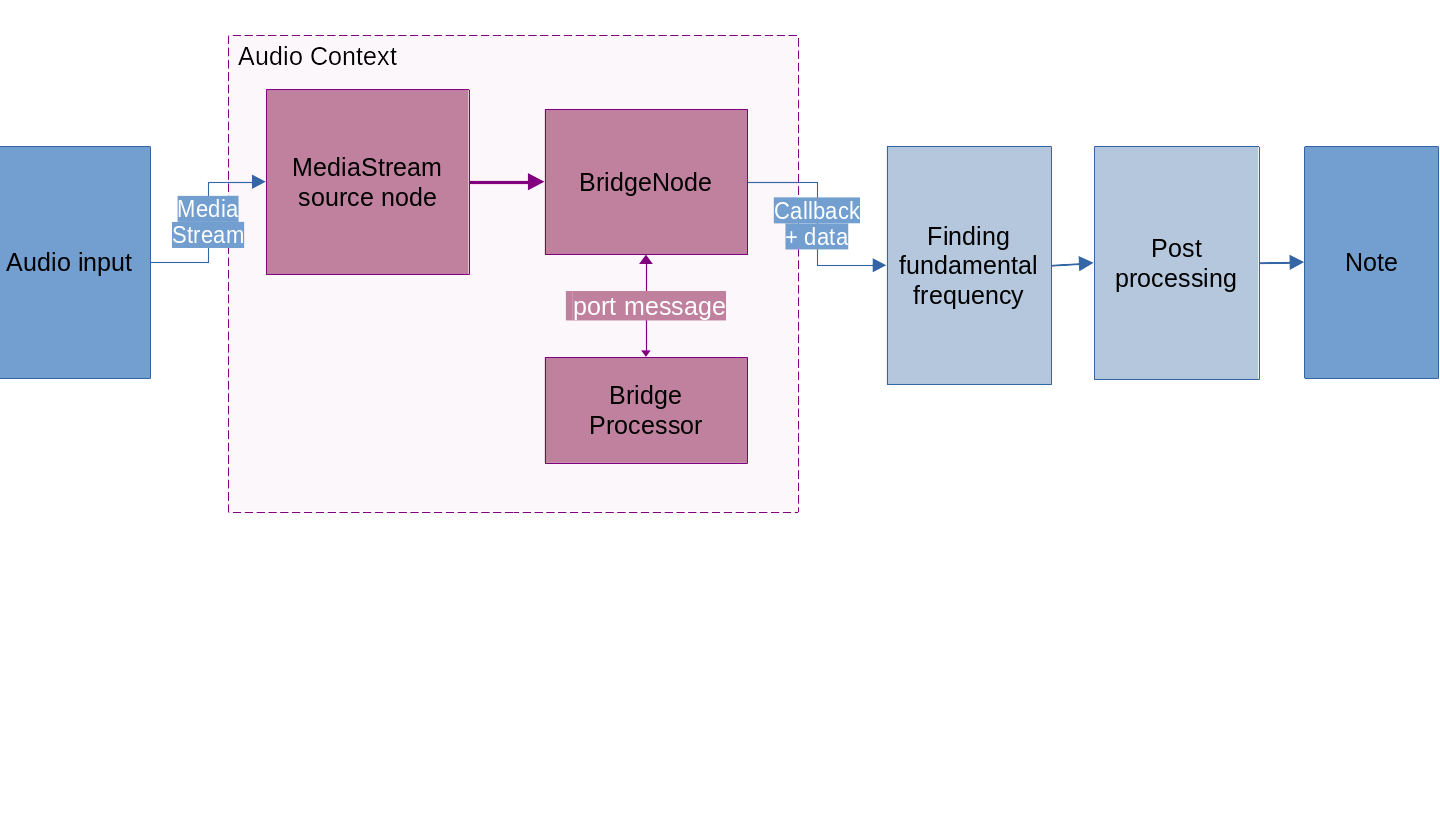
\includegraphics[width=\textwidth]{./images/pdArchitecture.png}
    \caption{Architecture describing the pitch detector. Stream is converted to a data array by having a worklet node send the raw audio data through the node-processor port to be used on the main thread.\label{fig:pdArch}}
\end{figure}

The proposed architecture offers flexibility without being overly complicated. The audio graph may be used to change the input from a microphone to a recording for validation and testing. It would also be possible to apply a real-time time-domain low-pass filter between the input node and the bridge node, which would allow downsampling and, thus, smaller FFT windows if computational power is a constraint. 

\subsection{Implementing the pitch detector}
With a plan for the detector, the next step is to implement it. The implementation, based on the architecture can be roughly divided into 4 parts: recording an input, passing data between the threads, accumulating and performing analysis.

\subsubsection{Audio input}
As the application utilizes the audio graph, any one of the source nodes may be used to input data into the pitch detector. For development, a reliable source signal is of more value than my sad attempt at singing, so a series of mp3 files, some of which were provided by FSM were used with a MediaElementAudioSourceNode. The mp3 files provided by FSM were for some reason set up so that the dominant voice is alone on channel and the 3 others are on the other stereo channel. This is no problem for the audio node based application, we can simply put a channel splitting node between the source node and the detector bridge node, and connect the channel with the discrete part to the bridge.
\lstinputlisting[style=javascript]{../snippets/PitchDetector-B.js}

\subsubsection{Worklet nodes}
Audio worklet nodes are a method of implementing custom audio modifier and sources (for example, a white noise generator). In this work, an AudioWorklet node will be used to implement the BridgeNode. Worklet nodes involve two parts: the node which is used in the audio graph, and the processor which is responsible for the behavior in the audio rendering thread. These are linked together.

The code snippet below shows how the BridgeNode is implemented.
\lstinputlisting[style=javascript]{../snippets/BridgeNode-A.js}
The bridge node extends or inherits the AudioWorklet node class and methods are added. When the node receives data on its port, it just forwards it to a handler. The handler could do further processing on the data but for the moment only forwards it to the callback function in the pitch detector. The pitch detector callback function is the one responsible for accumulating samples, zero-padding etc.

As the BridgeNode does not override or specify anything new, it is really only a thin wrapper for an AudioWorkletNode which is evident by the constructor calling the super function, which invokes the parent class constructor. This just allows the user to create a BridgeNode as a opposed to a generic WorkletNode with a custom processor. This is arguably unnecessary, but can make the code nicer to read. The processor which is implicitly passed to the BridgeNode via the super constructor must be created as well.

\lstinputlisting[style=javascript]{../snippets/BridgeProcessor-A.js}

As the purpose is not to actually process anything on the audio thread, but rather to utilize the flexibility of the audio graph and have processing done elsewhere, the processor simply sends everything it receives over the port to its node. 

The only thing left to do is to instantiate the BridgeNode. What connects to it may be a microphone, an audio file, a gain node, a channel splitter, or anything else that may be useful for the pitch detection.
\lstinputlisting[style=javascript]{../snippets/PitchDetector-A.js}

\subsection{Collecting samples}
The bridge node's sole purpose is to move audio data between the audio rendering thread and the main thread. To do this, the node periodically triggers a callback function with one render quantum as an argument. The user can define their own callback function.

\lstinputlisting[style=javascript]{../snippets/PitchDetector-C.js}

This also just forwards the render quantum to an analyze function to keep the code organized. In the analyze function is where accumulation happens and where analysis starts. For accumulating the samples, a ring buffer is used. When the function receives a render quantum, it first copies all the samples to a buffer with an offset. The write offset is then incremented by the render quantum size, a constant of 128.

\begin{lstlisting}[style=javascript]
// Copy buffer chunk to fft input vector.
for (let i = 0; i < RENDER_QUANTUM_SIZE; i++) {
    this.fftInputBuffer[i + this.fftBufferIteratorOffset] = data[i];
}
this.fftBufferIteratorOffset += RENDER_QUANTUM_SIZE;

// Perform all the analysis once enough samples.
if (this.fftBufferIteratorOffset >= FFT_TARGET_SAMPLE_SIZE) {
 // Analysis code...
 this.fftBufferIteratorOffset = 0;
}
\end{lstlisting}
When enough samples have been accumulated, a threshold which can be tuned, the analysis starts and the buffer iterator offset is reset. After the offset is reset, the new render quanta start overwriting old render quanta. In a limited sense, this functions as a ring buffer. Because the entire buffer is read at once, this provides all the ring buffer functionality needed for the accumulation. 

\subsection{Finding the fundamental frequency}
When enough samples have been collected (set to 6000 while development and testing), the next step is to forward transform the signal into the frequency domain. The following function is called which runs a 16384-point FFT using a library called fft.js by GitHub user indutny, which claims to be “The fastest JS Radix-4/Radix-2 FFT implementation”. The function is also responsible for creating the spectrum by calculating the magnitude of each complex data point using the Pythagorean theorem. 

\lstinputlisting[style=javascript]{../snippets/analysis-D.js}

The output of fft.js is a single array with alternating magnitudes and phases, which is why the frequency-magnitude computations may look odd. The function is called from the main analysis method.

\begin{lstlisting}[style=javascript]
    const spectrum = getSpectrum(this.fftInputBuffer, FFT_WINDOW_SIZE);
\end{lstlisting}

The signal is implicitly zero-padded because the input array is instantiated with 0's and only a portion of them are assigned a value, precisely the first 6016 values, 6016 being the smallest multiple of the render quantum size (128) greater than the target sample size.

The spectrum is then passed on to a function which computes the HPS of the spectrum. The HPS algorithm is ported to JavaScript and looks like the following. 

\lstinputlisting[style=javascript]{../snippets/analysis-A.js}

The array is instantiated, not as 0's, but as 1's for the multiplicative nature of the HPS. This can be thought of as the identity array, which means that the act of copying the initial array may be done by the same loop as the other iterations, but with a downsampling factor of 1, or in other words, no downsampling.

\subsubsection{Checking the spectrum flatness}
While developing the system, it was revealed that the input waveform is not always very tonic and this gives a spectrum that has more noise than peaks. This seems to largely happen for two reasons. The first is the time between certain notes, when the singer either just pauses or takes a breath, resulting in complete noise. The second is that when a note is sustained and decays, it eventually loses its tonality, also resulting in noise. To prevent this, the application simply ignores the incoming data until the data is something that can be worked with. 

In code, the spectral flatness is first computed with a fairly typical method, the ratio of the geometric mean and the arithmetic mean, as shown in the snippet below.

\lstinputlisting[style=javascript]{../snippets/analysis-B.js}

If this value is under $0.6$ (a value found empirically), the spectrum is deemed good and is given to the HPS. If the value is greater, the spectrum is ignored. The effect is that a note is assumed to continue until another clear note is received by the system. This mitigates the problems of noise due to silence or decay because the system just holds on to the last proper note it got. 

\subsubsection{Checking outliers}
The presence of obvious outliers were also revealed in early testing while developing. There were times, when the pitch detector would for brief periods get MIDI numbers of 32 and 80, which are lower than the lowest male bass singers and higher than the highest female singers. These are filtered out in the same way as with non-flat spectra, by just ignoring the note. 

\subsection{Post-processing}
Post-processing here refers to everything that is done after the fundamental frequency is found. Checking for flatness and the outliers could be considered post-processing methods, but they are done as earlier in the pipeline because it would be unnecessary to compute the HPS on a bad spectrum. Post-processing is strictly not necessary for pitch detection, but may help in simplifying analysis relating to the fundamental frequency, like scoring the accuracy of the user's singing. Post-processing also helps the user understand better what they may be doing wrong as pure frequencies mean very little to humans. 

\subsubsection{MIDI number to semitone name}
A formula for the MIDI number was derived in the previous chapter. The derived formula cleanly translates into JavaScript, as shown in the following snippet.

\begin{lstlisting}[style=javascript]
    const midiNumber = Math.round(12*Math.log2(frequency/440) + 69);
\end{lstlisting}

The MIDI number is convenient, because it is a semitone, a simple integer and a standard, meaning it is easier to use for computation and analysis. However, for most people, the MIDI number means very little and anyone who has any background in music is already familiar with the existing notation. To convert the MIDI number to a note, two functions can be derived using known MIDI numbers and their corresponding note names. 

The typical way to label a musical pitch is with SPN, where a number and a letter represents the octave and position within the octave. This is familiar to people with a background in music, and it would be the desired format for a note at the presentation layer.

As the notes repeat every octave and an octave consists of 12 semitones, the index that will be used to find the note within an octave is congruent to the MIDI number modulo 12. The octave number is the largest multiple of 12 strictly less than the number, which means it can be computed by rounding down the result of the MIDI number divided by 12. For some reason, the MIDI numbers misalign with the octave numbers, C0 being MIDI 12, the octave is shifted down one more step. The MIDI numbers, however, do align with the semitones as we start from C as C0 is the 12th MIDI number (which is congruent to 0 mod 12).

\lstinputlisting[style=javascript]{../snippets/analysis-C.js}

The semitones were previously defined, but those were only the semitones for some diatonic scales. Most of the semitones will be identical across scales, but the sharps and flats must be adjusted to present the sung note's name appropriately. For example, for the E-flat minor key, the note name array would still start on C and would contain a D and an E, but the second element should be Db (b for flat) as the E-flat minor scale contains a D-flat instead of a C-sharp. At logic level, these are represented by the exact same MIDI number class, which is all the MIDI numbers 1 above a multiple of 12, but at the presentation layer, it makes a difference for someone able to read sheet music who would most likely react to the mismatch in notation. The reference material Finlandia is played in A-flat so the semitones for the A-flat key are hard coded in the application for testing purposes but parameterized for the note name function. In a proper application, the key could be inferred from the source (for example musicXML) and then the appropriate semitone name array is applied.

\begin{lstlisting}[style=javascript]
    const AflatScale = ["C", "Db", "D", "Eb", "E", "F", "Gb", "G", "Ab", "A", "B", "H"]
    const noteName = getNoteName(this.currentDetectedNote, AflatScale);
\end{lstlisting}

\subsection{Current detected note and sampling}
The system continuously performs the FFT, checks for analysis criteria, performs HPS and post-processing, and is completely independent of the pace of the reference. This means that the output of the system is essentially a stream as well. The proposed solution is outlined in figure \ref{fig:samplerArch} where the output stream is fed into a sampler to get a discrete sequence of notes. 

\begin{figure}[ht]
    \centering
    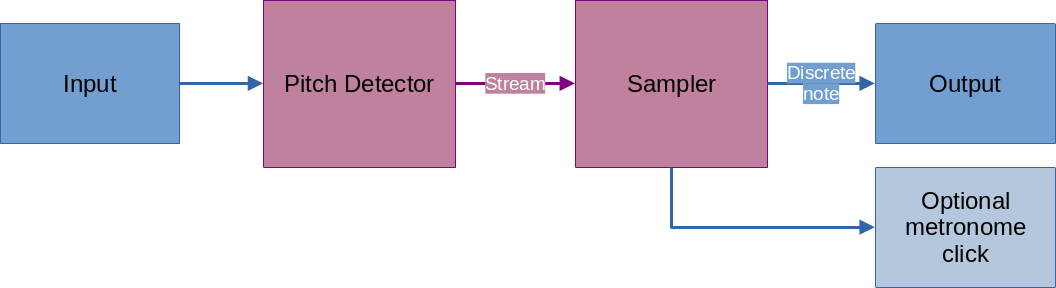
\includegraphics[width=\textwidth]{./images/samplerArch.png}
    \caption{Diagram of how a sampler interfaces with the system\label{fig:samplerArch}}
\end{figure}

An optional metronome could be added by triggering a click from the sampler. The click should not be triggered on every sample as multiple samples would likely be taken on every beat. 

The sampler subsystem is realized by continuously updating a single value in the pitch detector context and that value is checked by a function that is called periodically. For example, Finlandia's \textit{allegro} was first assumed to be around 120BPM and then timed to be close to this. The shortest notes in Finlandia are 8th notes which means that the system should sample frequently enough to catch 8th notes. If sampling happened on 4th notes, the system could only check the first of a pair of 8th notes. A minute is 60000 milliseconds, so the sampling interval should at the very least be $\frac{60000}{(8/4)*120} = 250ms$. This is the slowest pace at which Finlandia must be sampled without losing information.

Note that 250ms is not a latency that is added to the latency of the pitch detection. Assuming the timing is set up correctly between the metronome and the sampler, the sampler would catch the note the user is singing and give feedback instantly, it just would not give more feedback for another 250ms. This is likely acceptable because if the user can hit a note, they can likely also hold it for 250ms. Sampling faster would likely just give redundant feedback, however, this could be explored further. 

The values for these computations are once again hard coded. The snippet below shows how JavaScript is used to set up an interval that samples the continuously changing integer which represents the current detected note.  One approach to creating the metronome would be to have the sampler count to eight, trigger an audible (or visual) cue, then reset the count.

\lstinputlisting[style=javascript]{../snippets/PitchDetector-D.js}

